\documentclass[letterpaper]{article}
\usepackage[utf8]{inputenc}
\usepackage[parfill]{parskip}    % Activate to begin paragraphs with an empty line rather than an indent
\usepackage{graphicx}
\usepackage{amssymb}
\usepackage{amsmath}
\usepackage{amsthm}

\usepackage{afterpage}

\usepackage{algorithm}
\usepackage{algpseudocode}

\usepackage{verse}

\newtheorem{theorem}{Theorem}[section]
\newtheorem{corollary}{Corollary}[theorem]
\newtheorem{lemma}[theorem]{Lemma}

\theoremstyle{remark}
\newtheorem*{remark}{Remark}

\usepackage{epstopdf}
\usepackage{circuitikz}
\usepackage[separate-uncertainty = true,multi-part-units=single]{siunitx}
\usepackage{booktabs}
\usepackage{enumitem}
\usepackage[toc,page]{appendix}
\usepackage{color}
\usepackage{pgfplots}
\usepackage{pgfplotstable}
\usepackage{caption}
\usepackage{subcaption}
\usepackage{url}
\usepackage{multirow}
\usepackage{makecell}
\usepackage[round]{natbib}   % omit 'round' option if you prefer square brackets
\usepackage{titling}
\usepackage{siunitx}

\usepackage{setspace}
% \doublespacing
\usepackage{float}


\pgfplotsset{compat=1.14}

%  Special math symbols
%       floor, ceiling, angled brackets
%-----------------------------------------------------------------------
\newcommand{\floor}[1]{\left\lfloor #1\right\rfloor}
\newcommand{\ceil}[1]{\left\lceil #1\right\rceil}
\newcommand{\etal}{\textit{et al.}}
\newcommand{\RE}{\mathbb{R}}        % real space
\newcommand{\ZZ}{\mathbb{Z}}        % integers
\newcommand{\NN}{\mathbb{N}}        % natural numbers
\newcommand{\eps}{{\varepsilon}}    % prettier epsilon
%-----------------------------------------------------------------------
%  Tighter lists
%-----------------------------------------------------------------------
\newenvironment{itemize*}% Tighter itemized list
  {\begin{itemize}%
    \setlength{\itemsep}{-0.5ex}%
    \setlength{\parsep}{0pt}}%
  {\end{itemize}}
\newenvironment{description*}% Tighter description list
  {\begin{description}%
    \setlength{\itemsep}{-0.5ex}%
    \setlength{\parsep}{0pt}}%
  {\end{description}}
\newenvironment{enumerate*}% Tighter enumerated list
  {\begin{enumerate}%
    \setlength{\itemsep}{-0.5ex}%
    \setlength{\parsep}{0pt}}%
  {\end{enumerate}}
%-----------------------------------------------------------------------
% Typing shortcuts
%-----------------------------------------------------------------------
\newcommand{\X}{\mathbb{X}}
\newcommand{\SG}{\mathbf{S}}
\newcommand{\GE}{\mathcal{G}}
\newcommand{\ST}{\,:\,}
\renewcommand{\tilde}[1]{\widetilde{#1}}
\newcommand{\diam}{\mathrm{diam}}
\newcommand{\sq}{\square}
\newcommand{\half}[1]{\frac{#1}{2}}
\newcommand{\inv}[1]{\frac{1}{#1}}
\newcommand{\alg}{\textsf{SplitReduce}}
\newcommand{\sz}[1]{\sigma_{#1}}
\newcommand{\LL}{\mathcal{L}}
\newcommand{\softOmega}{\widetilde{\Omega}} 
\newcommand{\softO}{\widetilde{O}}
\newcommand{\OO}{O^*}  %or \widetilde{O}?

\newcommand{\norm}[1]{\left\lVert#1\right\rVert}

\newcommand{\dx}{\mathrm{d}x}
\newcommand{\dy}{\mathrm{d}y}
\newcommand{\dz}{\mathrm{d}z}
\newcommand{\dt}{\mathrm{d}t}
\newcommand{\du}{\mathrm{d}u}
\newcommand{\dtheta}{\mathrm{d}\theta}
\newcommand{\dq}{\mathrm{d}q}
\newcommand{\diff}{\mathrm{d}}
\newcommand{\dV}{\mathrm{d}V}
\newcommand{\dL}{\mathrm{d}L}
\newcommand{\dA}{\mathrm{d}A}
\newcommand{\dH}{\mathrm{d}H}
\newcommand{\df}{\mathrm{d}f}
\newcommand{\dg}{\mathrm{d}g}
\newcommand{\dr}{\mathrm{d}r}
\newcommand{\dw}{\mathrm{d}w}
\newcommand{\dv}{\mathrm{d}v}

\newcommand*\len[1]{\overline{#1}}

\newcommand{\dd}{Decadent Dwight cookies }
\newcommand{\hh}{Heavenly Hearst cookies }

\newcommand\note[1]{\marginpar{\textcolor{red}{#1}}}
\newcommand*{\tageq}{\refstepcounter{equation}\tag{\theequation}}

\newcommand*{\equals}{=}

\usepackage{fancyhdr}

\pgfplotscreateplotcyclelist{grayscale}{
    thick,white!10!black,mark=x,mark options=solid, dashed\\%
    thick,white!20!black,mark=o,mark options=solid\\%
}

\newcommand{\mat}[1]{\ensuremath{\begin{bmatrix}#1\end{bmatrix}}}
\newcommand{\eqn}[1]{\begin{alignat*}{2}#1\end{alignat*}}
\newcommand{\p}[2]{\frac{\partial #1}{\partial #2}}
\newcommand*{\thus}{&\implies\quad&}

\newcommand{\answer}[1]{\framebox{$\displaystyle #1 $}}

 
\pagestyle{fancy}
\fancyhf{}
\rhead{Rahul Arya}
\lhead{EE 16B}
\cfoot{\thepage}

\title{Lecture 2 - Notes}
\author{Rahul Arya}
\date{January 2019}
\begin{document}

\maketitle

\section{CMOS Capacitance and Homogeneous Linear Differential Equations}
So far, we have viewed CMOS transistors as components with either $0$ or infinite resistance, depending on the voltage between their gate and the source. However, in reality, they possess some internal resistance between the source and the drain, even when current is flowing. Moreover, there exists some capacitance between the gate and source, regardless of the state of the transistor. Thus, we can view a CMOS transistor as follows:
\begin{center}
\begin{circuitikz}[american] 
\draw (0, 0) node[ocirc]{} node[above]{$G$} to[C] (0, -2) to (1, -2) node[ocirc]{} node[below]{$S$} to[switch] (1, 0) to[R] (1, 2) node[ocirc]{} node[above]{$D$};
\end{circuitikz}
\end{center}

Putting two of these transistors together to form a CMOS inverter, we obtain
\begin{center}
\begin{circuitikz}[american] 
\draw (0, 2) to[C, l^=$C$] (0, 5) to (1, 5) to[switch] (1, 4) to[R, l=$R$] (1, 2);
\draw (0, 2) to[C, a=$C$] (0, -1) to (1, -1) to[switch] (1, 0) to[R, a=$R$] (1, 2);
\draw (-1, 2) node[ocirc]{} node[left]{IN} to (0, 2);
\draw (1, 2) to (3, 2) node[ocirc]{} node[right]{OUT};
\draw (2.3, 2) to[C, l=$C_{wire}$] (2.3, 0) node[ground]{};
\draw (1, -1) node[ground]{};
\draw (1, 5) to (1, 5.5) node[above]{$V_{dd}$};
\end{circuitikz}
\end{center}

We will show that these resistances and capacitances effectively add a \emph{delay} to CMOS circuits, so changes to the input will take some time to ``propagate" to the output. Note that the wire leading to the OUT terminal also has some capacitance to ground. In fact, in modern transistors, that capacitance is larger than the capacitance between the gate and the source. Thus, to obtain a more complete picture, we will consider two inverters connected together, as follows:
\begin{center}
\begin{circuitikz}[american] 
\draw (0, 2) to[C, l^=$C$] (0, 5) to (1, 5) to[switch] (1, 4) to[R, l=$R$] (1, 2);
\draw (0, 2) to[C, a=$C$] (0, -1) to (1, -1) to[switch] (1, 0) to[R, a=$R$] (1, 2);
\draw (-1, 2) node[ocirc]{} node[left]{IN} to (0, 2);
\draw (1, 2) to (3, 2);
\draw (2.3, 2) to[C, l=$C_{wire}$] (2.3, 0) node[ground]{};
\draw (1, -1) node[ground]{};
\draw (1, 5) to (1, 5.5) node[above]{$V_{dd}$};

\draw (4, 2) to[C, l^=$C$] (4, 5) to (5, 5) to[switch] (5, 4) to[R, l=$R$] (5, 2);
\draw (4, 2) to[C, a=$C$] (4, -1) to (5, -1) to[switch] (5, 0) to[R, a=$R$] (5, 2);
\draw (3, 2) to (4, 2);
\draw (5, 2) to (8, 2) node[ocirc]{} node[right]{OUT};
\draw (6.3, 2) to[C, l=$C_{wire}$] (6.3, 0) node[ground]{};
\draw (5, -1) node[ground]{};
\draw (5, 5) to (5, 5.5) node[above]{$V_{dd}$};
\end{circuitikz}
\end{center}

However, we will only analyze the first inverter. We will first consider the case when the first inverter starts with the input connected to ground, with the system as a whole in steady state. From the previous lecture, we know that the first output terminal will be outputting a logical $1$, and so is at voltage $V_{dd}$. Right now, the lower left switch (of the NMOS transistor) is open, and the upper left switch (of the PMOS transistor) is closed. 

At time $t = 0$, we connect the input to $V_{dd}$. The lower switch immediately closes, and the upper switch immediately opens. Thus, deleting disconnected components and other components that do not directly affect the first inverter, we obtain the following circuit:
\begin{center}
\begin{circuitikz}[american] 
\draw (1, -1) to[ncs] (1, 0) to[R, a=$R$] (1, 2);
\draw (2.3, 2) to[C, l=$C_{wire}$] (2.3, 0) node[ground]{};
\draw (3, 2) to (5, 2);
\draw (5, 2) to[C, l=$C$] (5, 4) node[above]{$V_{dd}$};
\draw (5, 2) to[C, l=$C$] (5, 0) node[ground]{};
\draw (1, -1) node[ground]{};
\draw (1, 2) to (3, 2) node[ocirc]{} node[above]{OUT};
\end{circuitikz}
\end{center}

It can be shown that we can rearrange the remaining capacitors into a single equivalent capacitance $C_{eq}$, to obtain the circuit:
\begin{center}
\begin{circuitikz}[american] 
\draw (1, -1)node[ground]{} to[ncs] (1, 0) to[R, a=$R$] (1, 2);
\draw (2.3, 2) to[C, l=$C_{eq}$, v=$ $] (2.3, -1) node[ground]{};
\draw (1, 2) to[short, i=$I$] (3, 2) node[ocirc]{} node[right]{OUT};
\end{circuitikz}
\end{center}

Let $Q(t)$ be the charge on the capacitor (following passive sign convention). Thus, by KVL and the capacitor equation $Q = VC$, moving counterclockwise around the circuit, we obtain
\[
    0 = I(t)R + \frac{Q(t)}{C_{eq}}.
\]
Let $V_C(t)$ be the voltage across the capacitor (and also the voltage at the output terminal). From Ohm's Law,
\eqn{
    && I(t)R &= 0 - V(t) \\
    &&&= -V(t) \\
    \thus I(t) &= -\frac{V(t)}{R}.
}
From the capacitor equation,
\eqn{
    && Q(t) &= C_{eq}V(t) \\
    \thus I(t) &= C_{eq} \frac{\dV}{\dt}.
}
Combining these two results for $I(t)$, we obtain
\eqn{
    && C_{eq} \frac{\dV}{\dt} &= -\frac{V(t)}{R} \\
    \thus \frac{\dV}{\dt} &= -\frac{1}{RC_{eq}}V(t).
}
Thus, we have obtained a first order homogeneous linear differential equation for the voltage at the output terminal. Recall that the initial output voltage was $V(0) = V_{dd}$, since the first inverter previously had its input connected to ground.

Solving using known techniques, we obtain
\eqn{
    && \frac{1}{V(t)} \dV &= -\frac{1}{RC_{eq}} \\
    \thus \ln{V(t)} - \ln{V(0)} &= -\frac{t}{RC_{eq}} \\
    \thus V(t) &= V(0) e^{-t/(RC_{eq}} \\
    \thus V(t) &= V_{dd} e^{-t/(RC_{eq})}.
}
We call the quantity $RC_{eq}$, which has units of time, the \emph{time constant} $\tau$ of this circuit. Thus, we can write the output voltage as
\[
    V(t) = V_{dd} e^{-t/\tau},
\]
which is the form in which it is most commonly seen. Plotting this function,
\begin{center}
\begin{tikzpicture}
\begin{axis}[
    xmin=0, xmax=5,
    ymin=0, ymax=1,
    xlabel=$t / \tau$, ylabel=$V(t) / V_{dd}$,
]
\addplot [domain=0:5, samples=10] {e^(-x)};
\end{axis}
\end{tikzpicture}
\end{center}
we see that it tends rapidly to $0$ (which is the steady state solution of an inverted with the input voltage set to a logical $1$), but never actually reaches it.

From the formula, we also see that every $\tau$ units of time, the voltage gets closer to the target voltage $0$ by a constant. After $\tau$ seconds, $V(t)$ drops to $0.37 V_{dd}$. After $3\tau$ seconds, $V(t)$ drops to $0.05 V_{dd}$. And after $7\tau$ seconds, $V(t)$ drops to $0.001 V_{dd}$, which we can treat as $0$ for all practical purposes.

It may be conjectured at this stage that this resistance and capacitance business doesn't really matter, since $V(t)$ approaches the target voltage very quickly. However, this behavior is only true for values of $t$ of the order of $\tau$. Looking at just the early portion of this graph ($0 \le t \le \tau / 5$),
\begin{center}
\begin{tikzpicture}
\begin{axis}[
    xmin=0, xmax=0.2,
    ymin=0, ymax=1,
    xlabel=$t / \tau$, ylabel=$V(t) / V_{dd}$,
]
\addplot [domain=0:5, samples=10] {e^(-x)};
\end{axis}
\end{tikzpicture}
\end{center}
we see that $V(t)$ barely drops from its initial value of $V_{dd}$, so the importance of these capacitive effects really depends on the time scales that we are working in.

\section{Inhomogeneous Differential Equations}
We can obtain similar results in the case of an inverter switching from an input of logical $1$ to logical $0$. Skipping over some steps, we obtain the equivalent circuit
\begin{center}
\begin{circuitikz}[american] 
\draw (1, -1)node[below]{$V_{dd}$} to[ncs] (1, 0) to[R, a=$R$] (1, 2);
\draw (2.3, 2) to[C, l=$C_{eq}$, v=$ $] (2.3, -1) node[ground]{};
\draw (1, 2) to[short, i=$I$] (3, 2) node[ocirc]{} node[right]{OUT};
\end{circuitikz}
\end{center}
More precisely, using the same variable definitions as before and following a similar approach, we obtain the differential equation
\[
    \frac{\dV}{\dt} = \frac{1}{RC_{eq}}(V_{dd} - V(t)).
\]
This equation is an \emph{inhomogeneous} linear first order differential equation. We say it is inhomogeneous because there is a constant term, in addition to the $V(t)$ and $\frac{\dV}{\dt}$ terms. To solve this equation, one way is to come up with a substitution for $V(t)$ that makes the equation homogeneous. Here, we will guess the substitution
\eqn{
    && V_{\Delta}(t) &= V(t) - V_{dd} \\
    \thus \frac{\dV_\Delta}{\dt} &= \frac{\dV}{\dt}.
}
Making the substitution, we obtain a homogeneous differential equation, which we can solve using standard techniques to obtain
\eqn{
    && \frac{\dV_\Delta}{\dt} &= -\frac{1}{RC_{eq}}V_\Delta(t) \\
    && \frac{1}{V_\Delta(t)} \dV &= -\frac{1}{RC_{eq}} \, \dt \\
    \thus \ln{V_\Delta(t)} - \ln{V_\Delta(0)} &= -\frac{t}{RC_{eq}} \\
    \thus V_\Delta(t) &= V_\Delta(0) e^{-t/(RC_{eq}} \\
    &&&= V_\Delta(0) e^{-t/\tau}
}

Since the input to the inverter was initially at logical $1$ for $t < 0$, the output started at logical $0$, so we have that $V(0) = 0$. Thus, $V_\Delta(0) = -V_{dd}$. Substituting into our solution for the differential equation, we obtain
\eqn{
    && V_\Delta(t) &= V_\Delta(0) e^{-t/\tau} \\
    \thus V(t) - V_{dd} &= -V_{dd}e^{-t /\tau} \\
    \thus V(t) &= V_{dd} (1 - e^{-t/\tau}).
}
Thus, we observe similar behavior to before, with $V(t)$ starting at $0$ and approaching $V_{dd}$ in the limit, but never quite reaching it.

\section{Propagation Delay}
Let's now look at a simpler circuit, with a resistor and capacitor in parallel, like so:
\begin{center}
\begin{circuitikz}[american] 
\draw (1, -1)node[below]{$V_{in}$} to (1, 0) to[R, a=$R$] (1, 2);
\draw (2.3, 2) to[C, l=$C_{eq}$, v=$ $] (2.3, -1) node[ground]{};
\draw (1, 2) to[short, i=$I$] (3, 2) node[ocirc]{} node[right]{$V_{out}$};
\end{circuitikz}
\end{center}
This circuit is fairly similar to the ones that we have previously looked at, except that there is no switch between the input voltage and the resistor. Now, we will set $V_{in}$ to a square wave, and observe the voltage $V_{out}$. Using techniques very similar to what we have previously used, we obtain a graph that looks like this:
\begin{center}
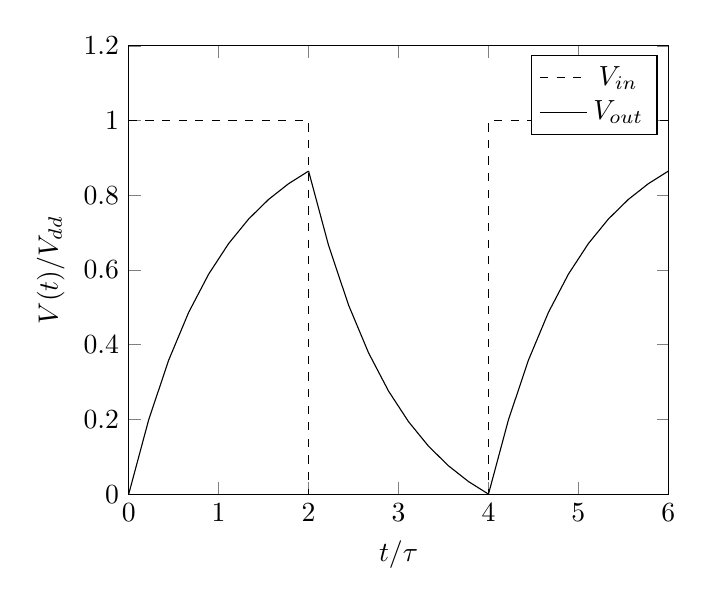
\begin{tikzpicture}
\begin{axis}[
    xmin=0, xmax=6,
    ymin=0, ymax=1.2,
    xlabel=$t / \tau$, ylabel=$V(t) / V_{dd}$,
]
\addplot [mark=none, dashed] coordinates {(0, 1) (2, 1) (2, 0) (4, 0) (4, 1) (6, 1)};
\addplot [domain=0:2, samples=10] {1 - e^(-x)};
\addplot [domain=2:4, samples=10] {-e^(-2) + e^(-(x - 2))};
\addplot [domain=4:6, samples=10] {1 - e^(-(x - 4))};

\addlegendentry{$V_{in}$}
\addlegendentry{$V_{out}$}
\end{axis}
\end{tikzpicture}
\end{center}

Intuitively, we can see that the capacitor causes $V_{out}$ to ``lag" behind $V_{in}$. 

This lag is one factor that limits the performance of more complex circuits. We wish to minimize the time constant $\tau$, in order to run our circuits at as high a frequency as possible. Recall that $\tau = RC$. We know that the capacitance of a capacitor is proportional to its area and inversely proportional to the distance between its plates. Thus, halving all dimensions of a capacitor will halve its capacitance, so by making transistors smaller, we can reduce their capacitance quite substantially. Although reducing the size of a resistor does not reduce its resistance, improvements in materials can again reduce the resistance of transistors quite substantially. 

However, this lag can also be beneficial, in creating timing circuits. Consider a circuit consisting of three inverters placed in series in a loop, as shown:
\begin{center}
\begin{circuitikz}[american] 
    \draw (0, 0) node[not port] (a1) {};
    \draw (2.5, 0) node[not port] (a2) {};
    \draw (5, 0) node[not port] (a3) {};
    \draw (a1.out) -- (a2.in);
    \draw (a2.out) -- (a3.in);
    \draw (a3.out) to (6, 0) to (6, 1) to (-1, 1) to (-1, 0) to (a1.in);
\end{circuitikz}
\end{center}

Imagine a logical $0$ input to the first inverter. This will feed a logical $1$ into the second inverter, a logical $0$ to the third, and finally a logical $1$ back to the first inverter. Thus, the voltage at the input to the first inverter (and at all other nodes in this circuit) will flip back and forth at a period based on the time constants of each of the inverters.

\section{Power Consumption}
The natural question to ask is: how fast can we make digital circuits, with today's technology? As it turns out, the limiting factor to circuit performance is not the time constant, but rather issues of heat dissipation. One circuit we can look at is a similar oscillating circuit consisting of $11$ such transistors with capacitances of \SI{10}{\femto\farad}, running at a frequency of \SI{10}{\giga\hertz} at a voltage of \SI{1}{\volt}. Clearly, each capacitor in each transistor will repeatedly be charged and discharged. When charged, each capacitor will store the energy
\[
    \frac{1}{2}QV = \frac{C}{2}V^2 \approx \SI{5}{\femto\joule}.
\]
It can also be easily calculated, using the techniques described above, that the energy lost to the resistor when charging the capacitor also equals $\frac{C}{2}V^2 \approx \SI{5}{\pico\joule}$. Thus, the net energy dissipated per cycle per transistor is
\[
    \Delta E = CV^2 \approx \SI{10}{\femto\joule}.
\]
Multiplying by the number of transistors (22) and the number of cycles per second (10 billion), we obtain a net power output of
\[
    22 \cdot \SI{10}{\giga\hertz} \cdot \SI{10}{\femto\joule} = \SI{2.2}{\milli\watt},
\]
with each transistor generating power of \SI{100}{\micro\watt}.

This is not very much. However, we must remember that the important measure to take into consideration is not the heat generated, but the heat generated per unit area. In order to achieve these frequencies, each transistor has an area of just \SI{2}{\micro\meter^2}, so the power density is
\[
    \frac{P}{A} = \frac{\SI{100}{\micro\watt}}{\SI{2}{\micro\meter^2}} = \SI{50}{\watt\milli\meter^{-2}}.
\]
This seems to be a much more impressive quantity. For comparison, the surface of the sun only has a heat flux of about \SI{25}{\watt\milli\meter^{-2}}!

This effect is a key factor in the cessation of Moore's law - while we continue to make increasingly smaller transistors, we become unable to cool their processors. So while we can make a \SI{10}{\giga\hertz} processor quite easily, we can't cool it!

\end{document}
